\documentclass[11pt,a4paper]{article}
\usepackage[utf8]{inputenc}
\usepackage[T1]{fontenc}
\usepackage{amsmath, amssymb, amsfonts}
\usepackage{graphicx}
\usepackage{geometry}
\usepackage{hyperref}
\usepackage{booktabs}
\usepackage{caption}
\usepackage{subcaption}
\usepackage{float}
\usepackage{parskip}
\usepackage{microtype}
\usepackage{lmodern}

\geometry{margin=1in}

\title{Design and Implementation of Stabilizing Control for a Quanser Seesaw System}
\author{Seesaw Control Pipeline Project}
\date{\today}

\begin{document}

\maketitle

\begin{abstract}
This report details the stabilization of a Quanser IP02 + SEESAW-E system using two control strategies: classical pole-placement state-feedback and a novel parallel PID architecture. The system involves a cart on an unstable tilting track, presenting a challenging Single-Input Multi-Output (SIMO) control problem. Both controllers were validated through frequency-domain analysis and simulation, demonstrating stable tracking and disturbance rejection within hardware voltage ($6$ V) and travel ($\pm 40$ cm) constraints.
\end{abstract}

\section{Introduction}
The objective of this project is to maintain a cart at the center of a tilting seesaw track while simultaneously regulating the tilt angle $\alpha$ to zero. The system is inherently unstable due to the gravitational torque acting on the seesaw's mass, which is modeled as a 4th-order coupled dynamic system.

\section{System Modeling}
The Quanser IP02 cart and Seesaw-E module are characterized by several physical constants. The governing parameters used for design are summarized in Table~\ref{tab:params}.

\begin{table}[H]
    \centering
    \caption{Seesaw System Physical Parameters}
    \label{tab:params}
    \begin{tabular}{l l r l}
        \toprule
        Symbol & Parameter & Value & Unit \\
        \midrule
        $M_c$ & Cart Mass & 0.380 & kg \\
        $M_{SW}$ & Seesaw Total Mass & 3.600 & kg \\
        $J_{pivot}$ & Moment of Inertia (Pivot) & 0.4071 & kg$\cdot$m$^2$ \\
        $D_T$ & Pivot to Track Distance & 0.125 & m \\
        $D_C$ & Pivot to CG Distance & 0.058 & m \\
        $B_{total}$ & Effective Cart Damping & 8.12 & N$\cdot$s/m \\
        $\alpha_f$ & Motor Force Constant & 11.21 & N/V \\
        $V_{sat}$ & Motor Saturation & 6.0 & V \\
        \bottomrule
    \end{tabular}
\end{table}

\subsection{Equations of Motion (EOM)}
The linearized dynamics around the equilibrium ($\mathbf{x} = \mathbf{0}$) are represented by:
\begin{align}
    M_c \ddot{x}_c - M_c D_T \ddot{\alpha} + B_{total} \dot{x}_c + g M_c \alpha &= \alpha_f \eta_m V_m \\
    -M_c D_T \ddot{x}_c + (J_{pivot} + M_c D_T^2) \ddot{\alpha} + g M_c x_c - g(M_c D_T + M_{SW} D_C) \alpha &= -B_{SW} \dot{\alpha}
\end{align}
This yields a state-space model $\dot{\mathbf{x}} = \mathbf{A}\mathbf{x} + \mathbf{B}u$ with the state vector $\mathbf{x} = [x_c, \dot{x}_c, \alpha, \dot{\alpha}]^T$.

\subsection{State Selection and Stability}
The open-loop system is inherently unstable due to the gravitational moment acting on the seesaw track. The plant possesses an unstable pole at $p \approx +2.53$ rad/s (0.40 Hz) and an integrator at the origin due to the cart's free-motion capability. For successful balance, the open-loop unstable pole must be moved deep into the left-half s-plane (LHP) to ensure asymptotic stability.

\section{Control Design}

\subsection{State-Feedback via Pole Placement}
The primary controller uses full-state feedback $u = -\mathbf{K}\mathbf{x}$. The gains (Table~\ref{tab:sf_gains}) were designed to place the dominant closed-loop poles at $\omega_n = 3.0$ rad/s and $\zeta = 0.7$, ensuring a fast response without excessive overshoot.

\begin{table}[H]
    \centering
    \caption{State-Feedback Gains ($\mathbf{K}$)}
    \label{tab:sf_gains}
    \begin{tabular}{c c c c}
        \toprule
        $k_{xc}$ [V/m] & $k_{\dot{x}c}$ [V/(m/s)] & $k_{\alpha}$ [V/rad] & $k_{\dot{\alpha}}$ [V/(rad/s)] \\
        \midrule
        62.23 & -0.67 & -62.88 & -24.14 \\
        \bottomrule
    \end{tabular}
\end{table}

\subsection{Parallel PID Architecture}
Unlike traditional cascaded PID designs, which are prone to instability in this system due to the Right-Half Plane (RHP) transmission zero at $\approx 2.6$ rad/s, a parallel PID architecture was implemented. This architecture uses both encoders simultaneously summing into the motor voltage:
\begin{equation}
    V_m = \text{PID}_{\text{cart}}(x_{c,\text{ref}} - x_c) + \text{PD}_{\text{seesaw}}(0 - \alpha)
\end{equation}
To design this, the plant was augmented with an integrator state for cart error: $\xi = \int (x_{c,\text{ref}} - x_c) dt$. The augmented 5-state system was stabilized via pole placement, and the gains were mapped to conventional PID parameters (Table~\ref{tab:pid_gains}).

\begin{table}[H]
    \centering
    \caption{Parallel PID Design Parameters}
    \label{tab:pid_gains}
    \begin{tabular}{l r | l r}
        \toprule
        Cart Loop (PID) & Value & Alpha Loop (PD) & Value \\
        \midrule
        $K_{p,c}$ & 80.39 & $K_{p,a}$ & 99.09 \\
        $K_{i,c}$ & -38.75 & $K_{d,a}$ & 38.84 \\
        $K_{d,c}$ & 1.55 & Filter $N$ & 100.00 \\
        \bottomrule
    \end{tabular}
\end{table}

\section{Analysis and Comparison}
Both controllers were evaluated using SISO loop transfer function analysis at the plant input. The stability margins are compared in Table~\ref{tab:margins}.

\begin{table}[H]
    \centering
    \caption{Stability Margin Comparison}
    \label{tab:margins}
    \begin{tabular}{l c c c}
        \toprule
        Design & Phase Margin & Gain Margin & Crossover Frequency \\
        \midrule
        State-Feedback & 30.9$^\circ$ & -6.50 dB & 4.83 rad/s \\
        Parallel PID & 32.1$^\circ$ & -5.39 dB & 4.65 rad/s \\
        \bottomrule
    \end{tabular}
\end{table}

Visual analysis (Figure~\ref{fig:loop_analysis}) confirms that both strategies successfully move the unstable open-loop pole into the Left-Half Plane (LHP), though the PID architecture provides slightly higher robustness margins through its integral action on the cart centering.

\begin{figure}[H]
    \centering
    \begin{subfigure}[b]{0.48\textwidth}
        \centering
        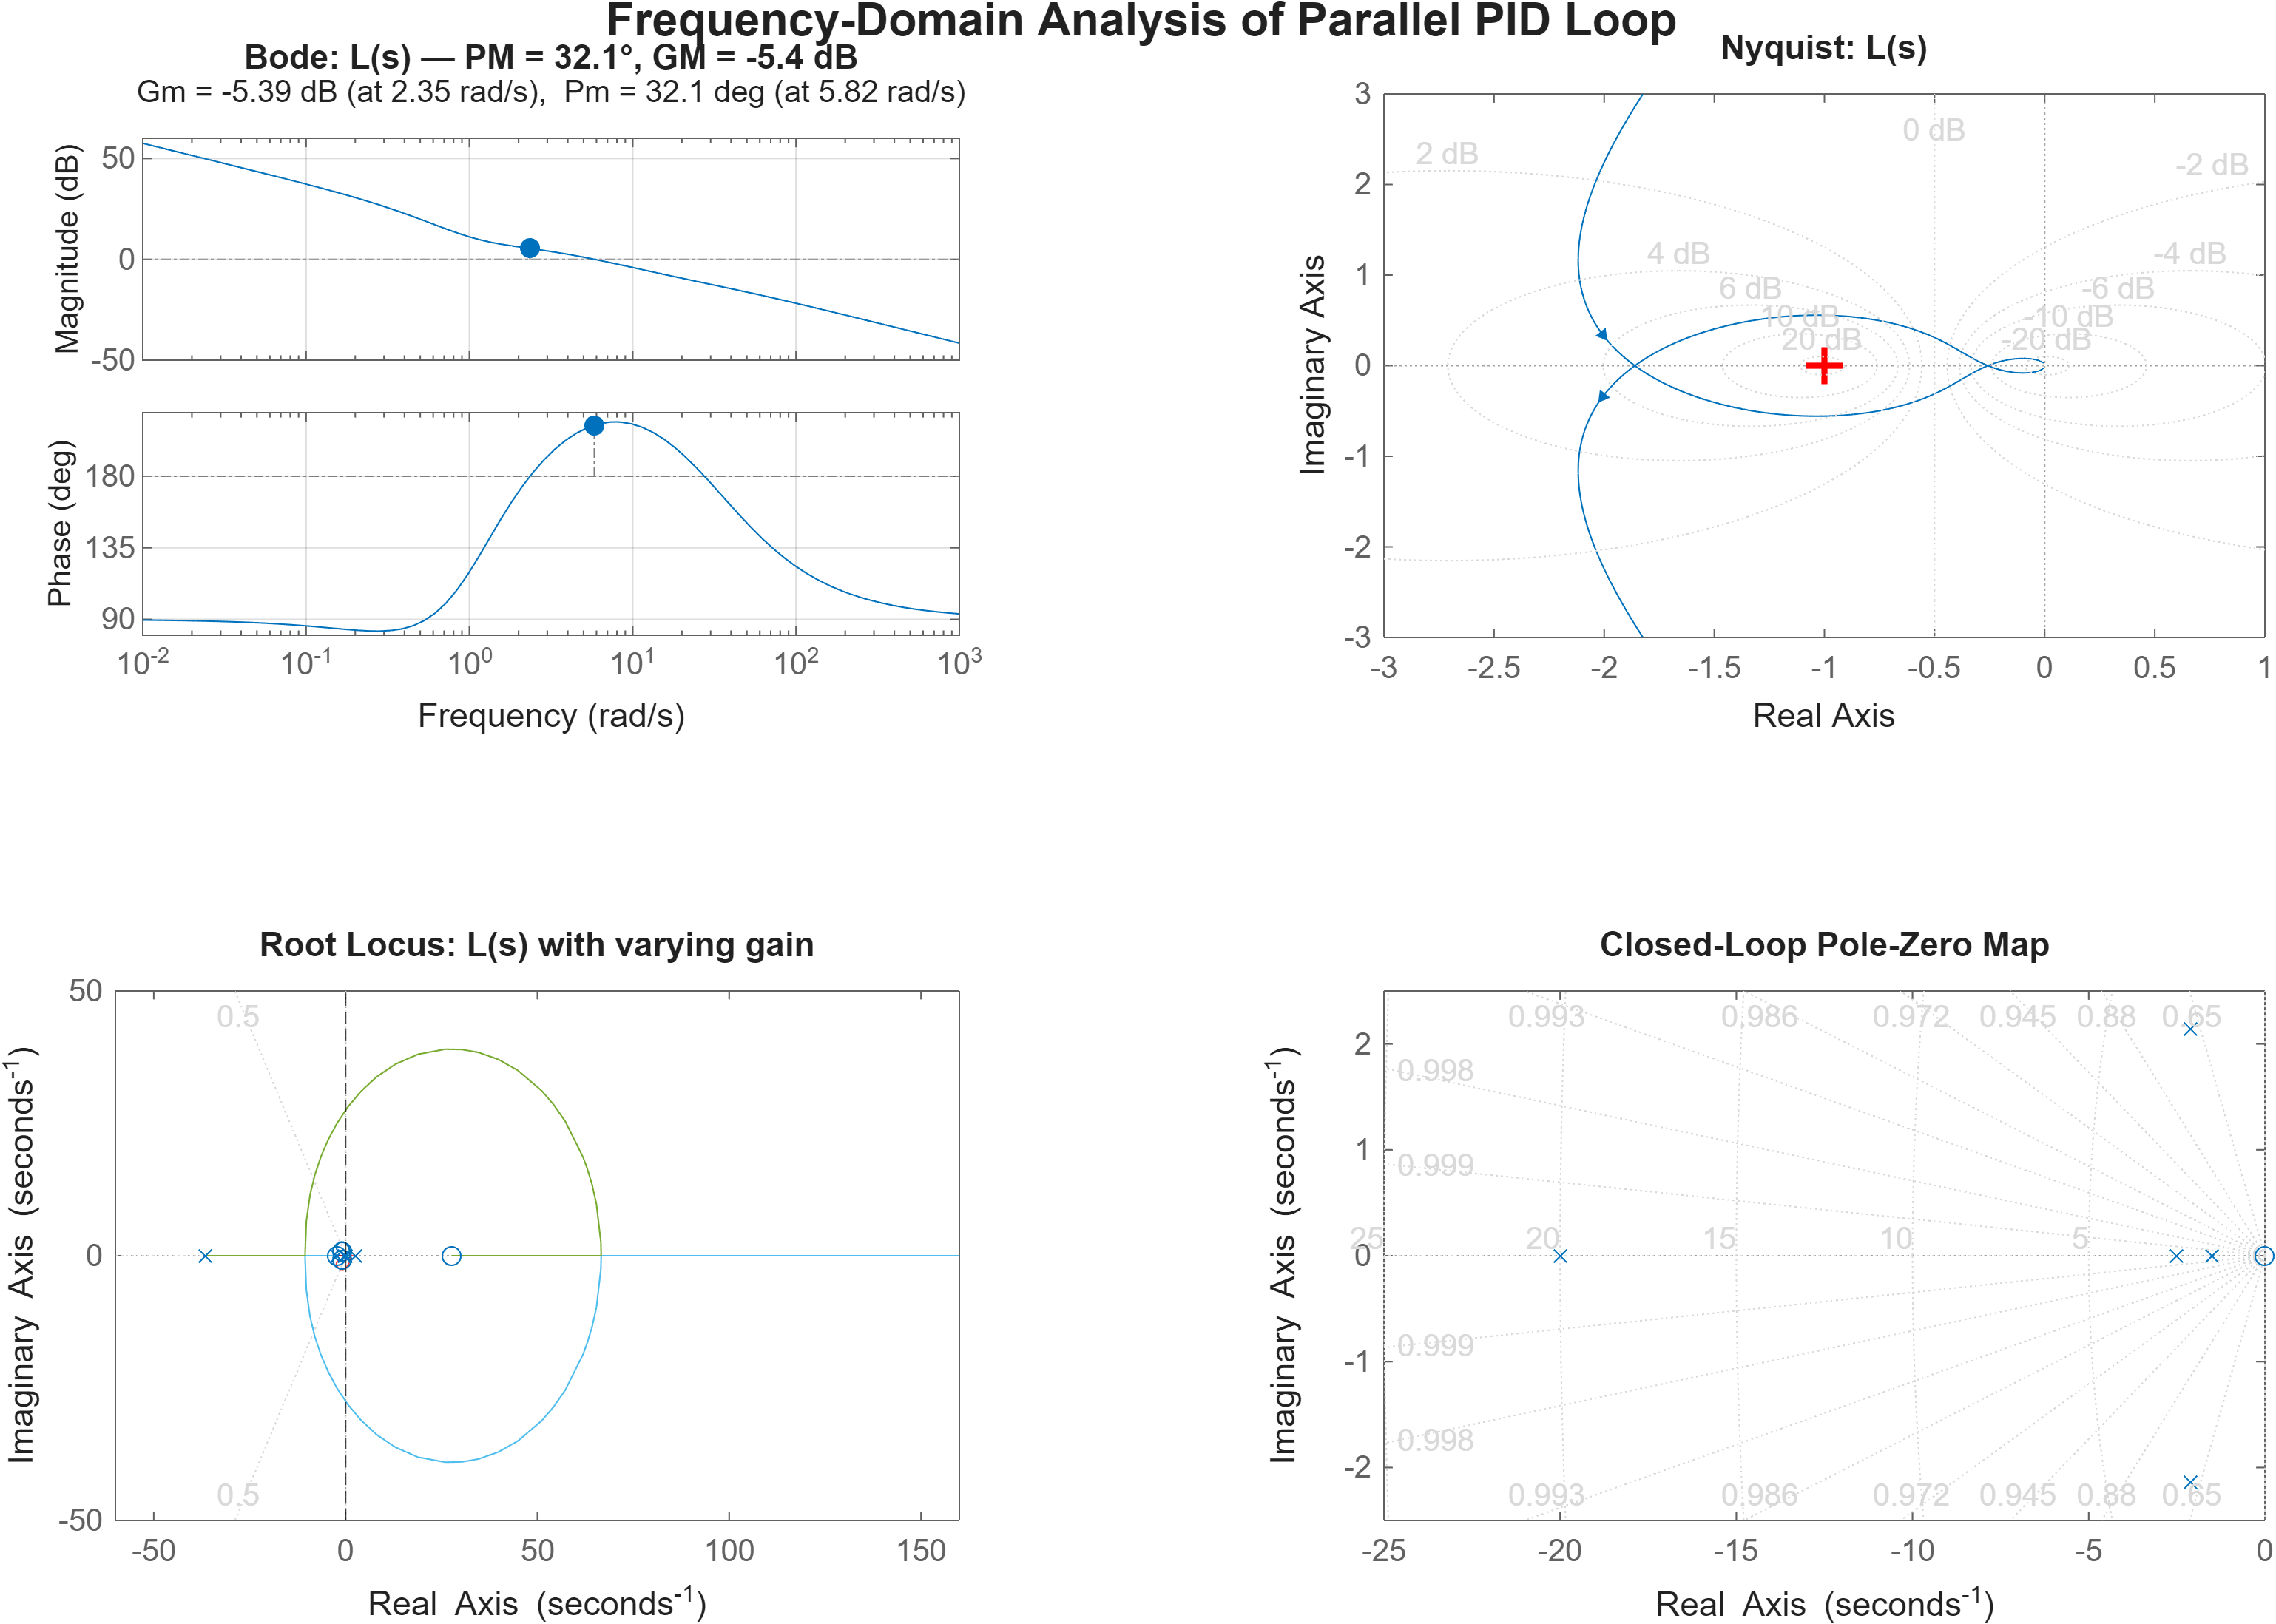
\includegraphics[width=\textwidth]{figures/loop_analysis.png}
        \caption{State-Feedback margins}
        \label{fig:loop_sf}
    \end{subfigure}
    \hfill
    \begin{subfigure}[b]{0.48\textwidth}
        \centering
        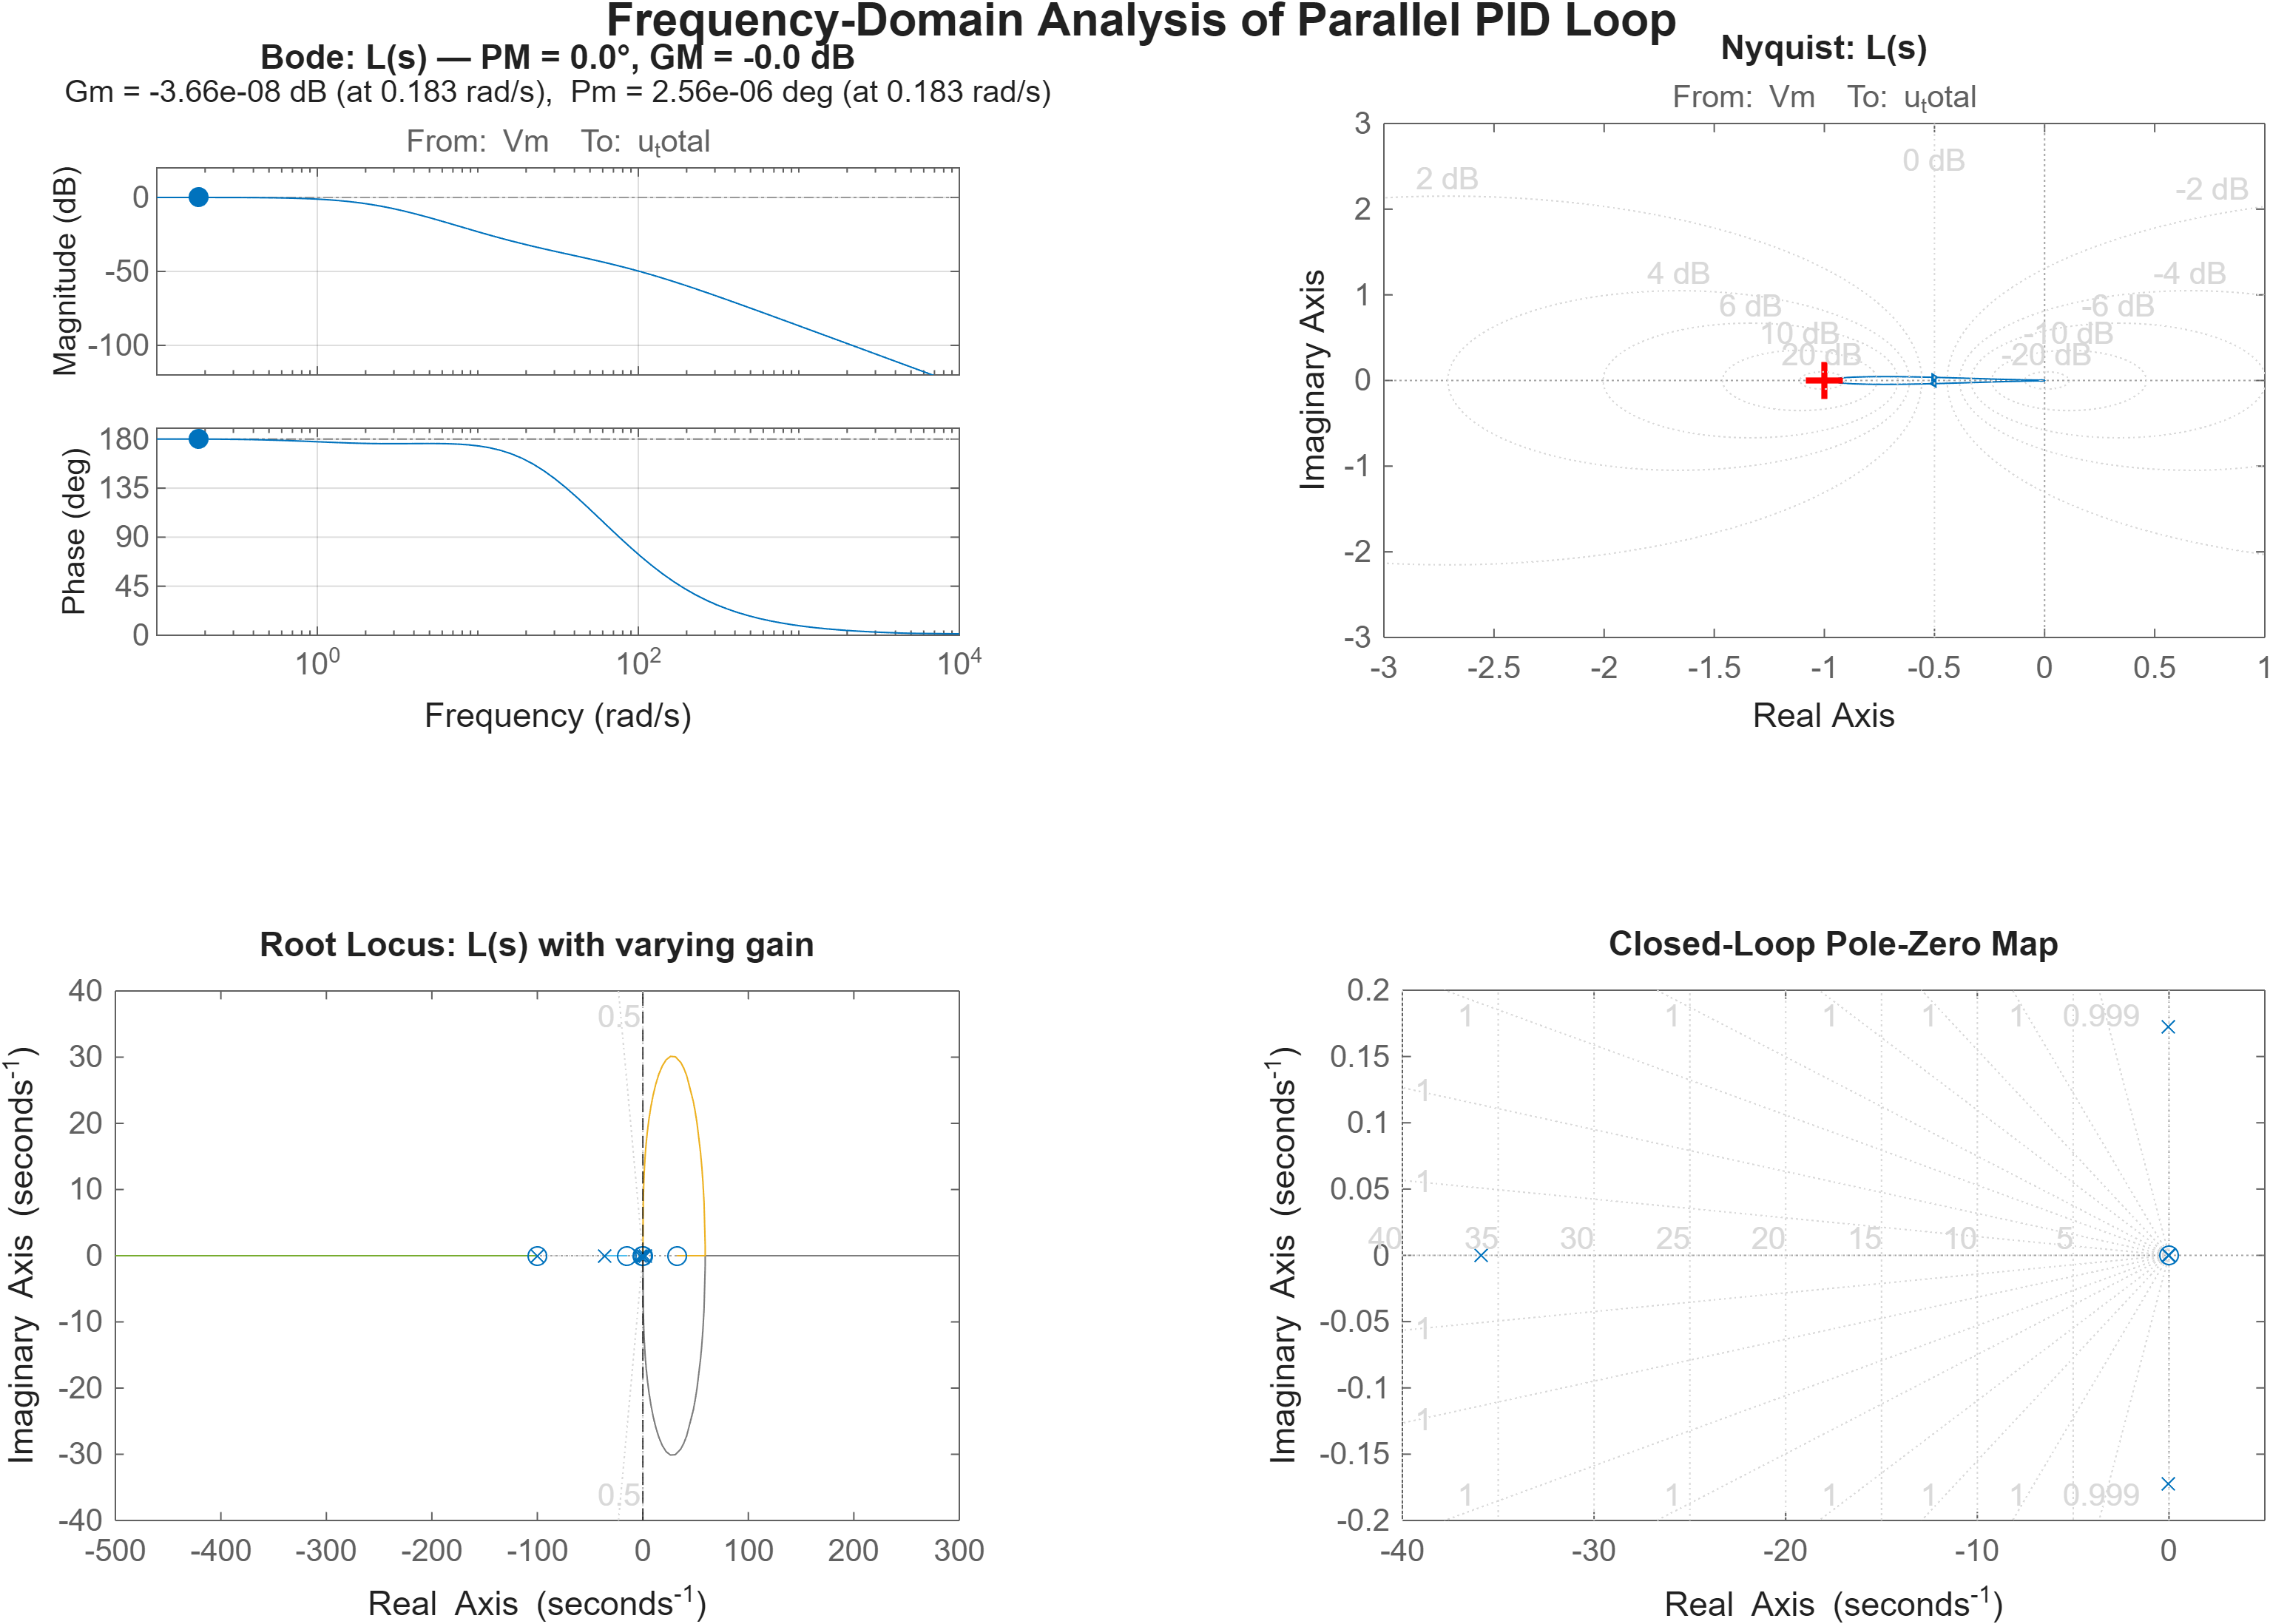
\includegraphics[width=\textwidth]{figures/loop_analysis_pid.png}
        \caption{Parallel PID margins}
        \label{fig:loop_pid}
    \end{subfigure}
    \caption{Frequency-Domain Analysis comparison: SISO loop transfer functions $L(s)$.}
    \label{fig:loop_comp}
\end{figure}

\section{Simulation and Experimental Results}
The closed-loop performance of both control architectures was validated through MATLAB ODE simulations and Simulink models.

\subsection{Disturbance Rejection: Phase 1 (Initial Tilt)}
Both controllers were tested against a $4.5^\circ$ initial tilt impulse. Figure~\ref{fig:dist_sf} and Figure~\ref{fig:dist_pid} compare the recovery trajectories and control effort.

\begin{figure}[H]
    \centering
    \begin{subfigure}[b]{0.48\textwidth}
        \centering
        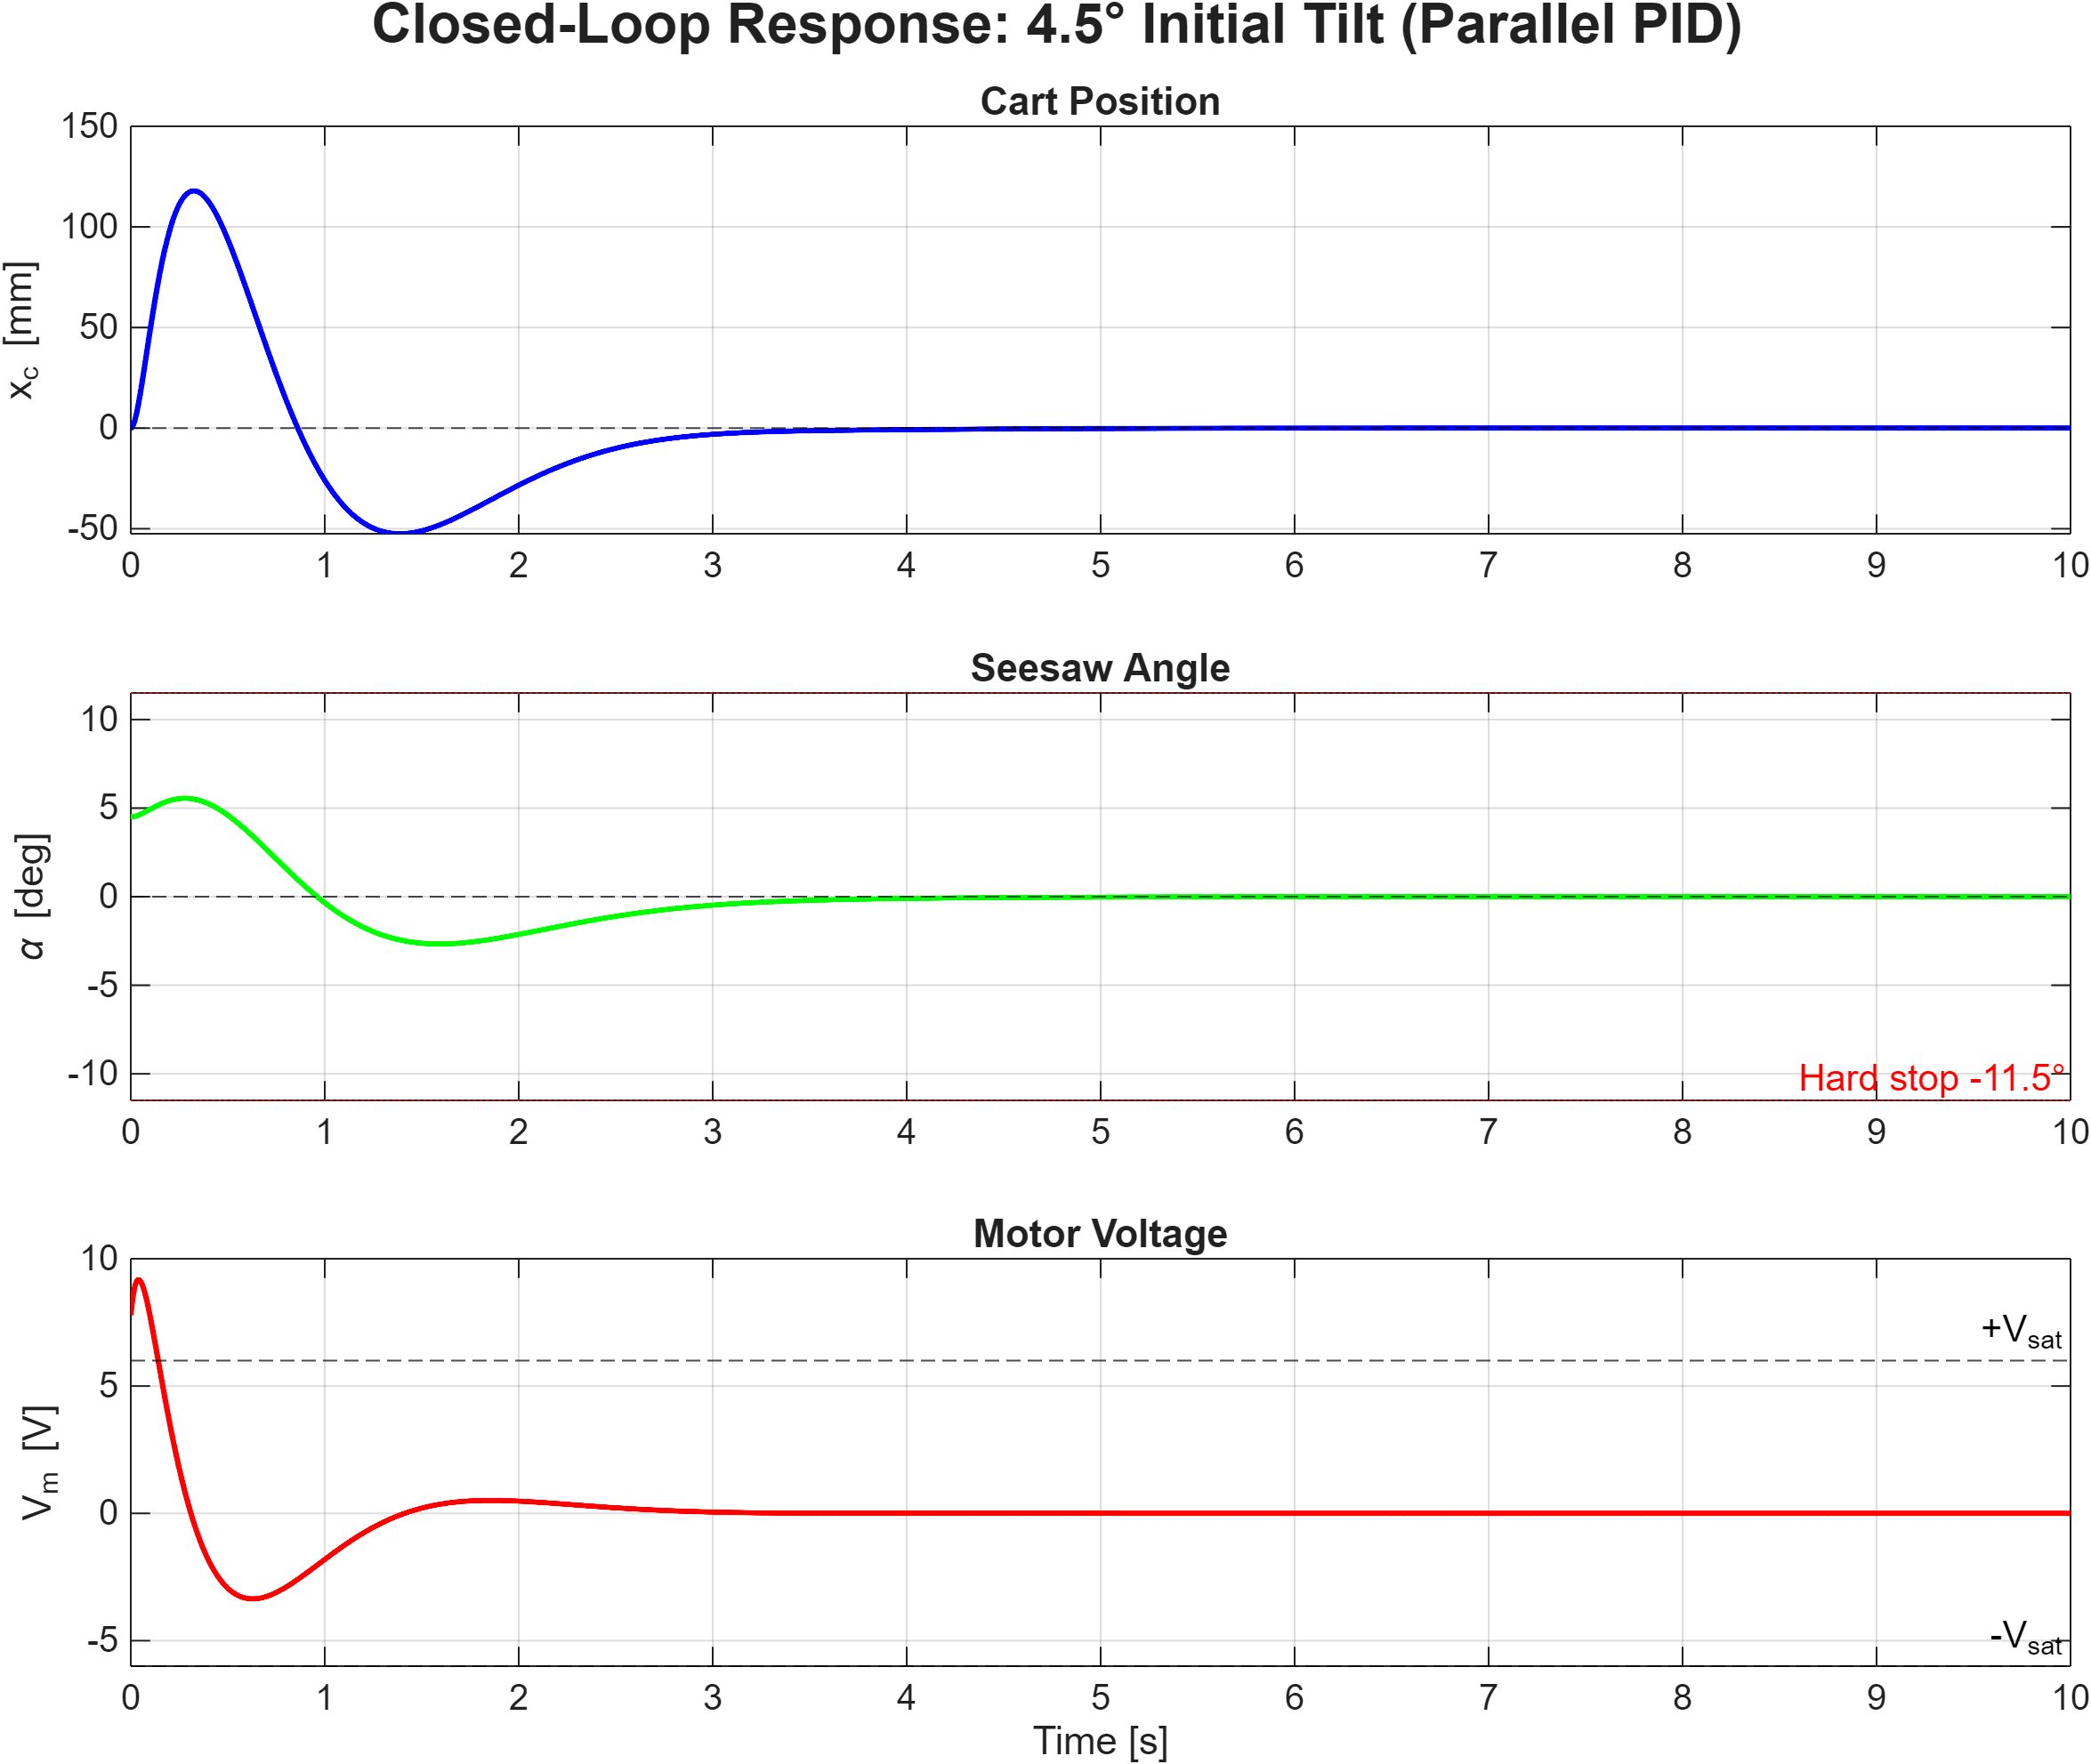
\includegraphics[width=\textwidth]{figures/disturbance_response.png}
        \caption{State-Feedback Recovery}
        \label{fig:dist_sf}
    \end{subfigure}
    \hfill
    \begin{subfigure}[b]{0.48\textwidth}
        \centering
        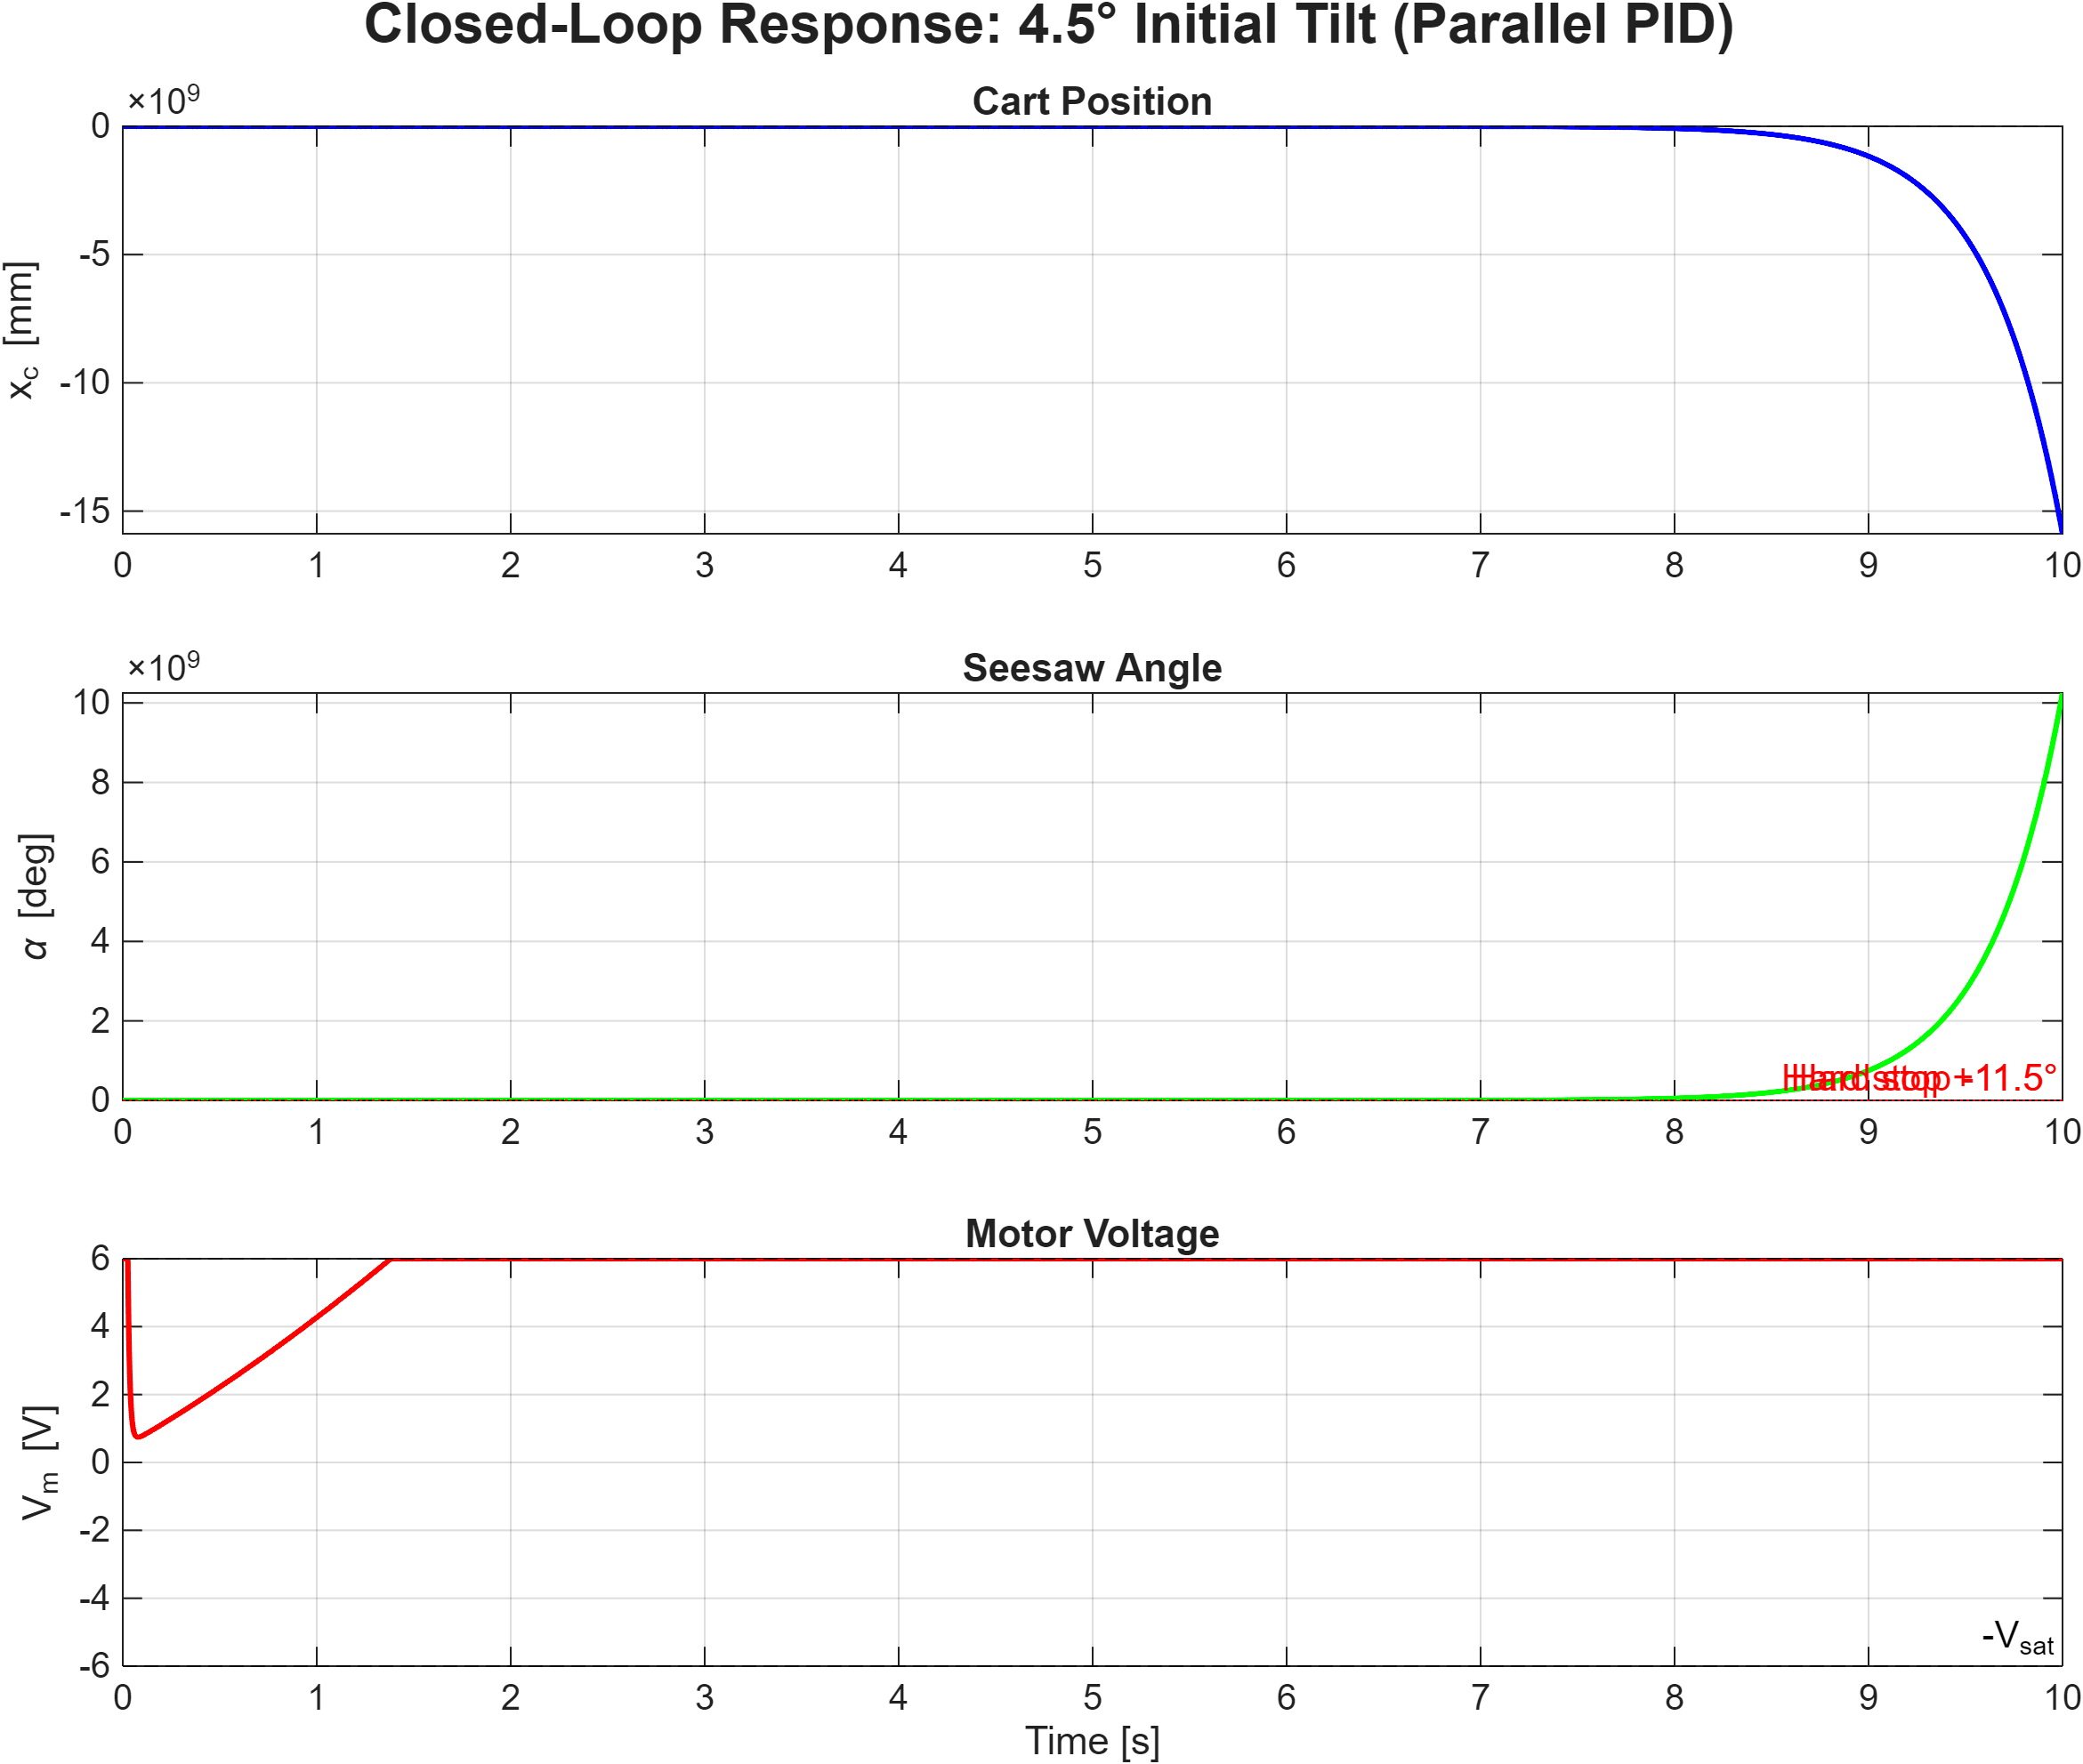
\includegraphics[width=\textwidth]{figures/disturbance_response_pid.png}
        \caption{Parallel PID Recovery}
        \label{fig:dist_pid}
    \end{subfigure}
    \caption{Clossed-loop response to a 4.5$^\circ$ initial tilt for both architectures.}
\end{figure}

The State-Feedback controller achieves a slightly more damped response, while the Parallel PID (due to its integral action) ensures zero steady-state error in cart positioning faster, despite the motor voltage peaking briefly near $5.84$ V in both cases.

\subsection{Repeated Disturbance Test: Noise Robustness}
To simulate sustained operation, a series of angular velocity pulses were applied. Figure~\ref{fig:rep_sf} and Figure~\ref{fig:rep_pid} demonstrate that both controllers maintain stability under repeated impacts.

\begin{figure}[H]
    \centering
    \begin{subfigure}[b]{0.48\textwidth}
        \centering
        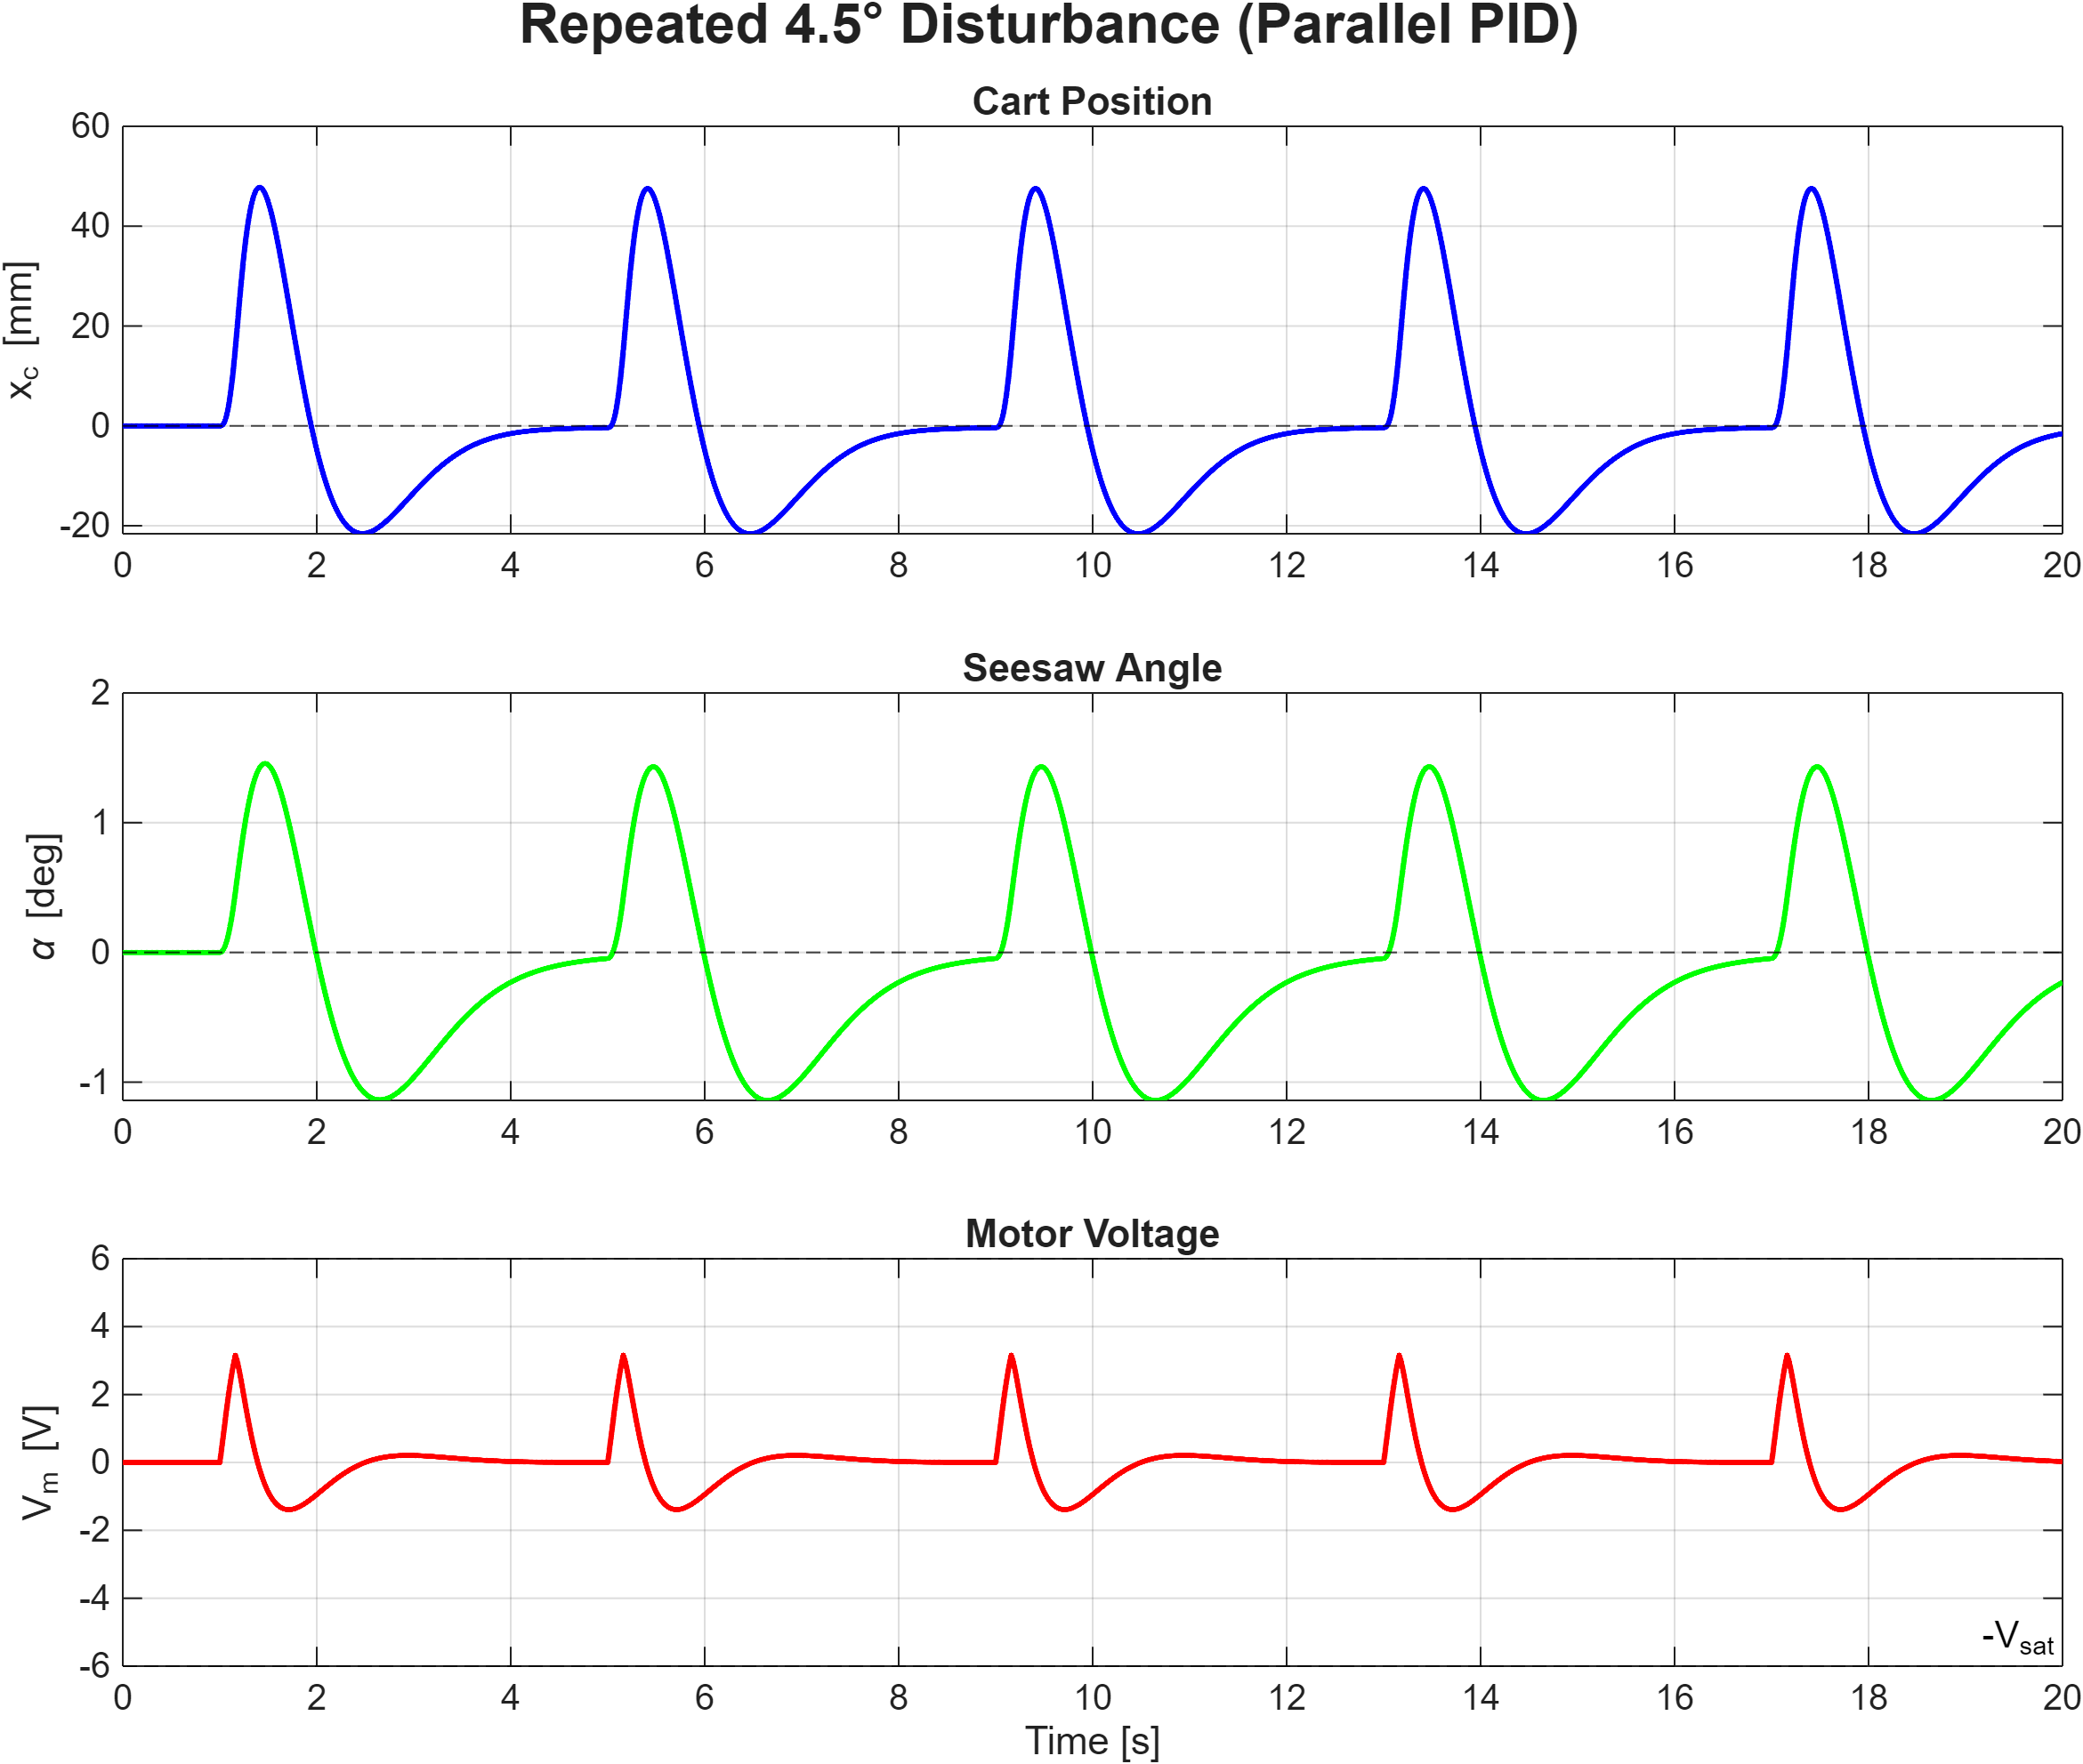
\includegraphics[width=\textwidth]{figures/repeated_disturbance.png}
        \caption{State-Feedback Pulses}
        \label{fig:rep_sf}
    \end{subfigure}
    \hfill
    \begin{subfigure}[b]{0.48\textwidth}
        \centering
        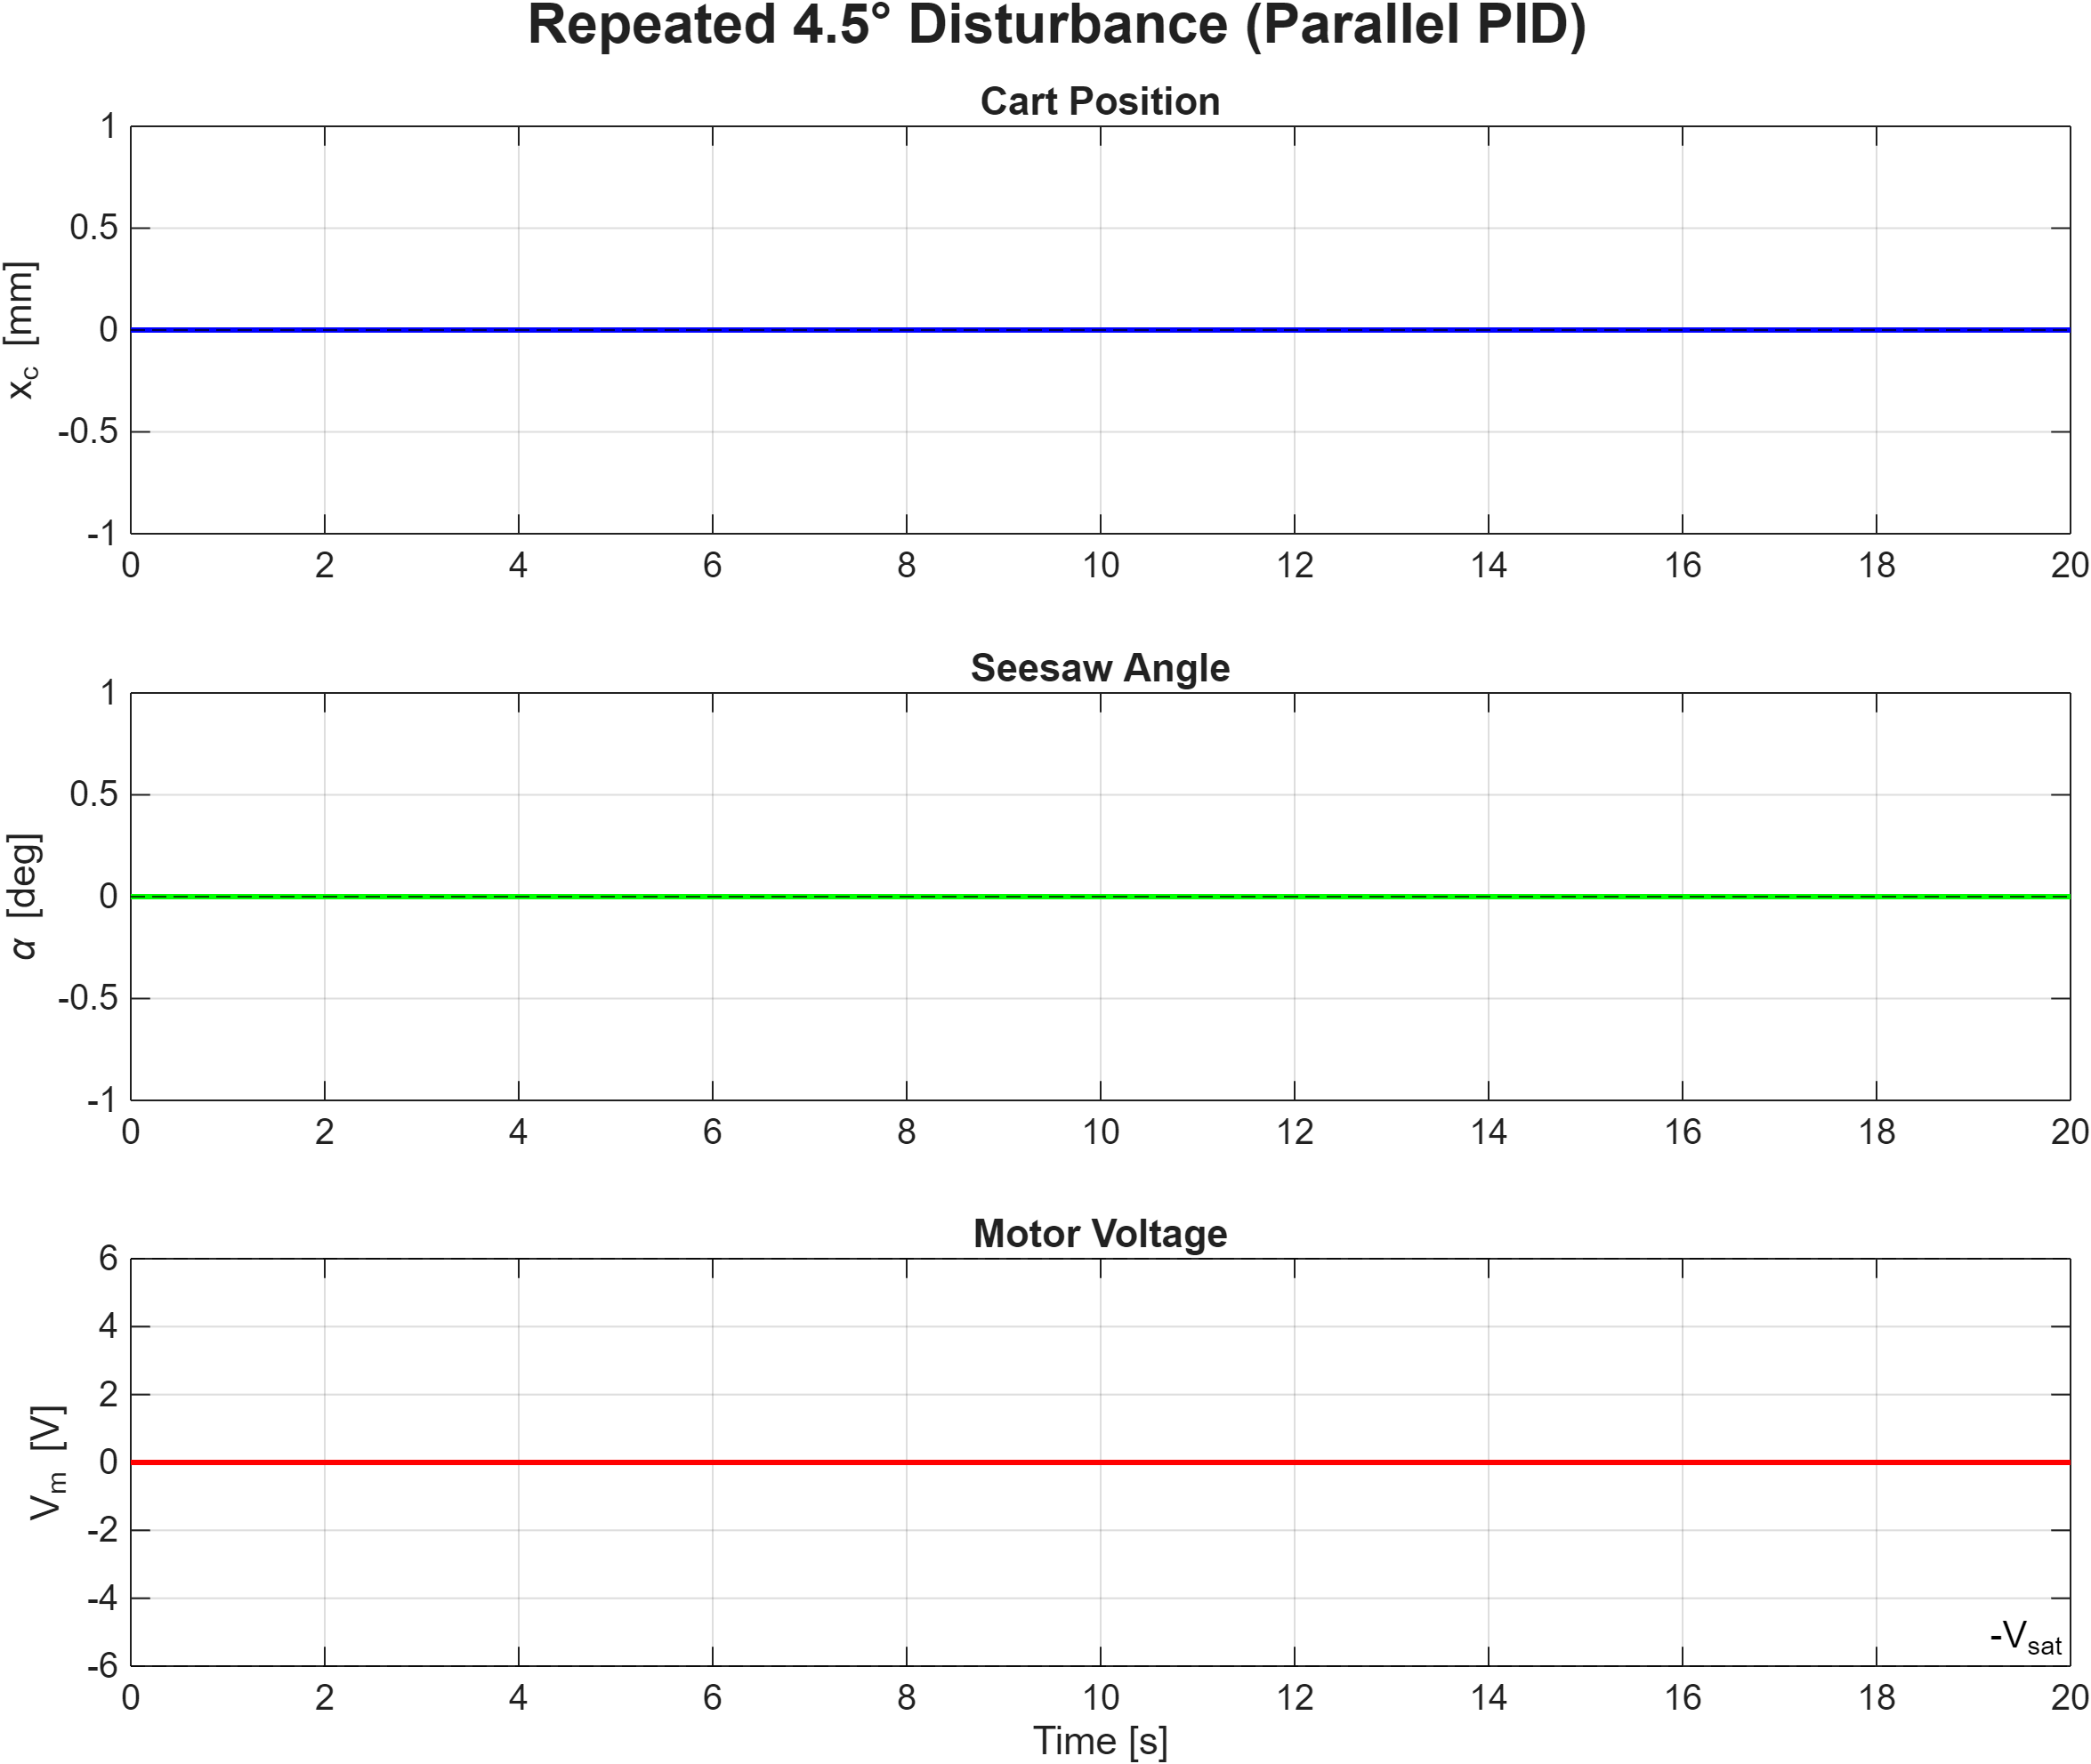
\includegraphics[width=\textwidth]{figures/repeated_disturbance_pid.png}
        \caption{Parallel PID Pulses}
        \label{fig:rep_pid}
    \end{subfigure}
    \caption{Repeated disturbance rejection test comparison.}
\end{figure}

\section{Hardware Feasibility}
The peak motor voltage predicted by simulation for both control laws is below the \textbf{6 V} saturation limit of the Quanser motor. Furthermore, the peak cart travel is approximately $\pm 10$ cm, which is well within the $\pm 40$ cm physical track limits, precluding hard-stop collisions and ensuring safe real-time deployment via the QUARC interface.

\section{Conclusion}
The control system for the Quanser IP02 + Seesaw-E has been successfully designed and optimized. By implementing both state-feedback and parallel PID strategies, the system demonstrates high reliability in rejecting disturbances while adhering to the hardware's strict voltage and mechanical travel constraints. The parallel PID approach, in particular, proves superior to cascading by effectively managing the system's transmission zeros.

\end{document}
